\chapter{Preliminary fits}
\label{chap:cpv:prelim_fits}

The yield extraction technique used to measure the signal yields entering the 
computation of \ARaw, shown in \cref{eqn:cpv:introduction:araw}, is described 
in \cref{chap:cpv:araw}.
Before then, it is useful to fit to the charge-combined data in order to 
perform studies that require background subtraction, selection efficiency 
estimates, and the like.
This \namecref{chap:cpv:prelim_fits} describes the binned \chisq\ fit to the 
\phh\ invariant mass spectrum that is used for such studies.

\section{Input data and shape parameterisation}
\label{chap:cpv:prelim_fits:data_pdfs}

The data entering the fit depends on the study that the information is needed 
for.
For example, the study of the optimal \ac{PID} requirements described in 
\cref{chap:cpv:selection:offline} requires a mass fit before the offline 
\ac{PID} requirements are applied.
In all cases, the models and general fit procedure are the same.

The mass spectrum of the three-body \phh\ system is used to discriminate 
between signal and background.
The following will list the functional forms used in the fit to describe the 
these components of the data.
In all cases, the normalisation factors are omitted from the definitions, and 
the variable $x$ represents the \PLambdac\ mass.

For both the \pKK\ and \ppipi\ samples, the signal model $f$ is the linear sum 
of two normal distributions $G$ sharing a common mean $\mu$ but with different 
widths $\sigma_{1}$ and $\sigma_{2}$.
A `single Gaussian' is defined as
\begin{equation}
  G(x; \mu, \sigma) = \exp\left(-\frac{{(x - \mu)}^{2}}{2\sigma^{2}}\right),
\end{equation}
and then the `double Gaussian' is defined as
\begin{equation}
  f(x; \mu, w, \alpha) = \alpha{}G(x; \mu, \alpha{w}) +
    (1 - \alpha)G(x; \mu, \frac{w}{\alpha}),
  \label{eqn:cpv:prelim_fits:sig_model}
\end{equation}
where $\alpha$ describes the `relative strength' of each normal distribution 
and is bounded in the range $[0, 1]$, and the widths $\sigma_{1}$ and 
$\sigma_{2}$ have been parameterised as
\begin{equation}
  \sigma_{1} = \alpha{w},\ \text{and}\ \sigma_{2} = \frac{w}{\alpha}.
  \label{eqn:cpv:prelim_fits:sigma_def}
\end{equation}
This enforces the relation $\sigma_{1} \leq \sigma_{2}$, which is useful to 
know when trying to reason about the fitted values of $\alpha$, and was 
observed to increase the stability of the fit compared to having free, 
independent widths $\sigma_{1}$ and $\sigma_{2}$.

For both modes, the background model $g$ is a first-order polynomial with 
coefficient $a_{0}$
\begin{equation}
  g(x) = 1 + a_{0}x.
  \label{eqn:cpv:prelim_fits:bkg_model}
\end{equation}

The signal and background models are combined as a linear sum to form a total 
function $h$, where each component is weighted by their respective yields 
\nsig\ and \nbkg
\begin{equation}
  h(x) = \nsig f(x) + \nbkg g(x).
\end{equation}
The \chisq\ fit is performed on the data by minimising a normalised version of 
$h$ in the range
\begin{equation}
  2230 < m(\PLambdac) < \SI{2350}{\GeV},
\end{equation}
with bins of width \SI{1}{\MeV}.

Once a fit has converged and the associated covariance matrix is confirmed to 
be positive-definite, sWeights~\cite{Pivk:2004ty} are computed and are attached 
to each candidate that entered the fit.
This allows for the statistical subtraction of either the signal or the 
background component in bins of some variable that is not correlated with the 
\PLambdac\ mass.

Fits to the fully selected 2012 magnet down dataset for the \pKK\ and \ppipi\ 
modes are given in \cref{fig:cpv:prelim_fits:full}.
The corresponding correlation matrices are given in 
\cref{fig:cpv:prelim_fits:full_correlation}, and the parameter values are given 
in \cref{tab:cpv:prelim_fits:params:pKK,tab:cpv:prelim_fits:params:ppipi}.
A good description of the data is seen, and this is representative of the fit 
quality in all data sub-samples.

Tables of signal and background yields measured in the preliminary fit are 
given for each fully selected subset of the data for \pKK\ in 
\cref{tab:cpv:prelim_fits:yields:pKK} and for \ppipi\ in 
\cref{tab:cpv:prelim_fits:yields:ppipi}.
Also given are the number of signal candidates per unit of integrated 
luminosity $\nsig/\intlumi$, where the integrated luminosity is given for each 
data subset in \cref{tab:cpv:data:luminosity}.

\section{Validation}
\label{chap:cpv:prelim_fits:validation}

To evaluate the bias and uncertainty coverage of the fitter, pseudo-experiments 
are performed by generating \ac{MC} data from the fitted \ac{PDF}.
One thousand pseudo-experiments are run for each mode and for each data 
sub-sample.
The parameter values of the generating \acp{PDF}, from which data points are 
drawn, are the same as those found in the fits to the fully selected data, 
except for the values of yield parameters.
Each yield parameter value for each pseudo-experiment is drawn from a Poisson 
distribution whose mean is set to the value of the yield found in the fits to 
the data~\cite{Karbach:2012vg}.

For each pseudo-experiment, the fitted parameter value and the uncertainty on 
that fit are recorded, and a pull value $p$ is computed as the difference 
between the fitted value $v'$ and the true generating value $v$, divided by the 
parameter value uncertainty $\unc{v}$
\begin{equation}
  p = \frac{v - v'}{\unc{v}}.
\end{equation}
The true value for each yield parameter is taken to be the mean value of the 
Poisson distribution from which the generating value is drawn.
An unbiased fitter with correct uncertainty coverage should have a distribution 
of pull values drawn from a unit Gaussian.

The results of the pseudo-experiments are shown in 
\cref{fig:cpv:prelim_fits:validation:pKK} and 
\cref{fig:cpv:prelim_fits:validation:ppipi} for the 2012 magnet down \pKK\ and 
\ppipi\ data.
It is seen that the signal yield parameter is unbiased.

\begin{figure}
  \begin{subfigure}[b]{0.5\textwidth}
    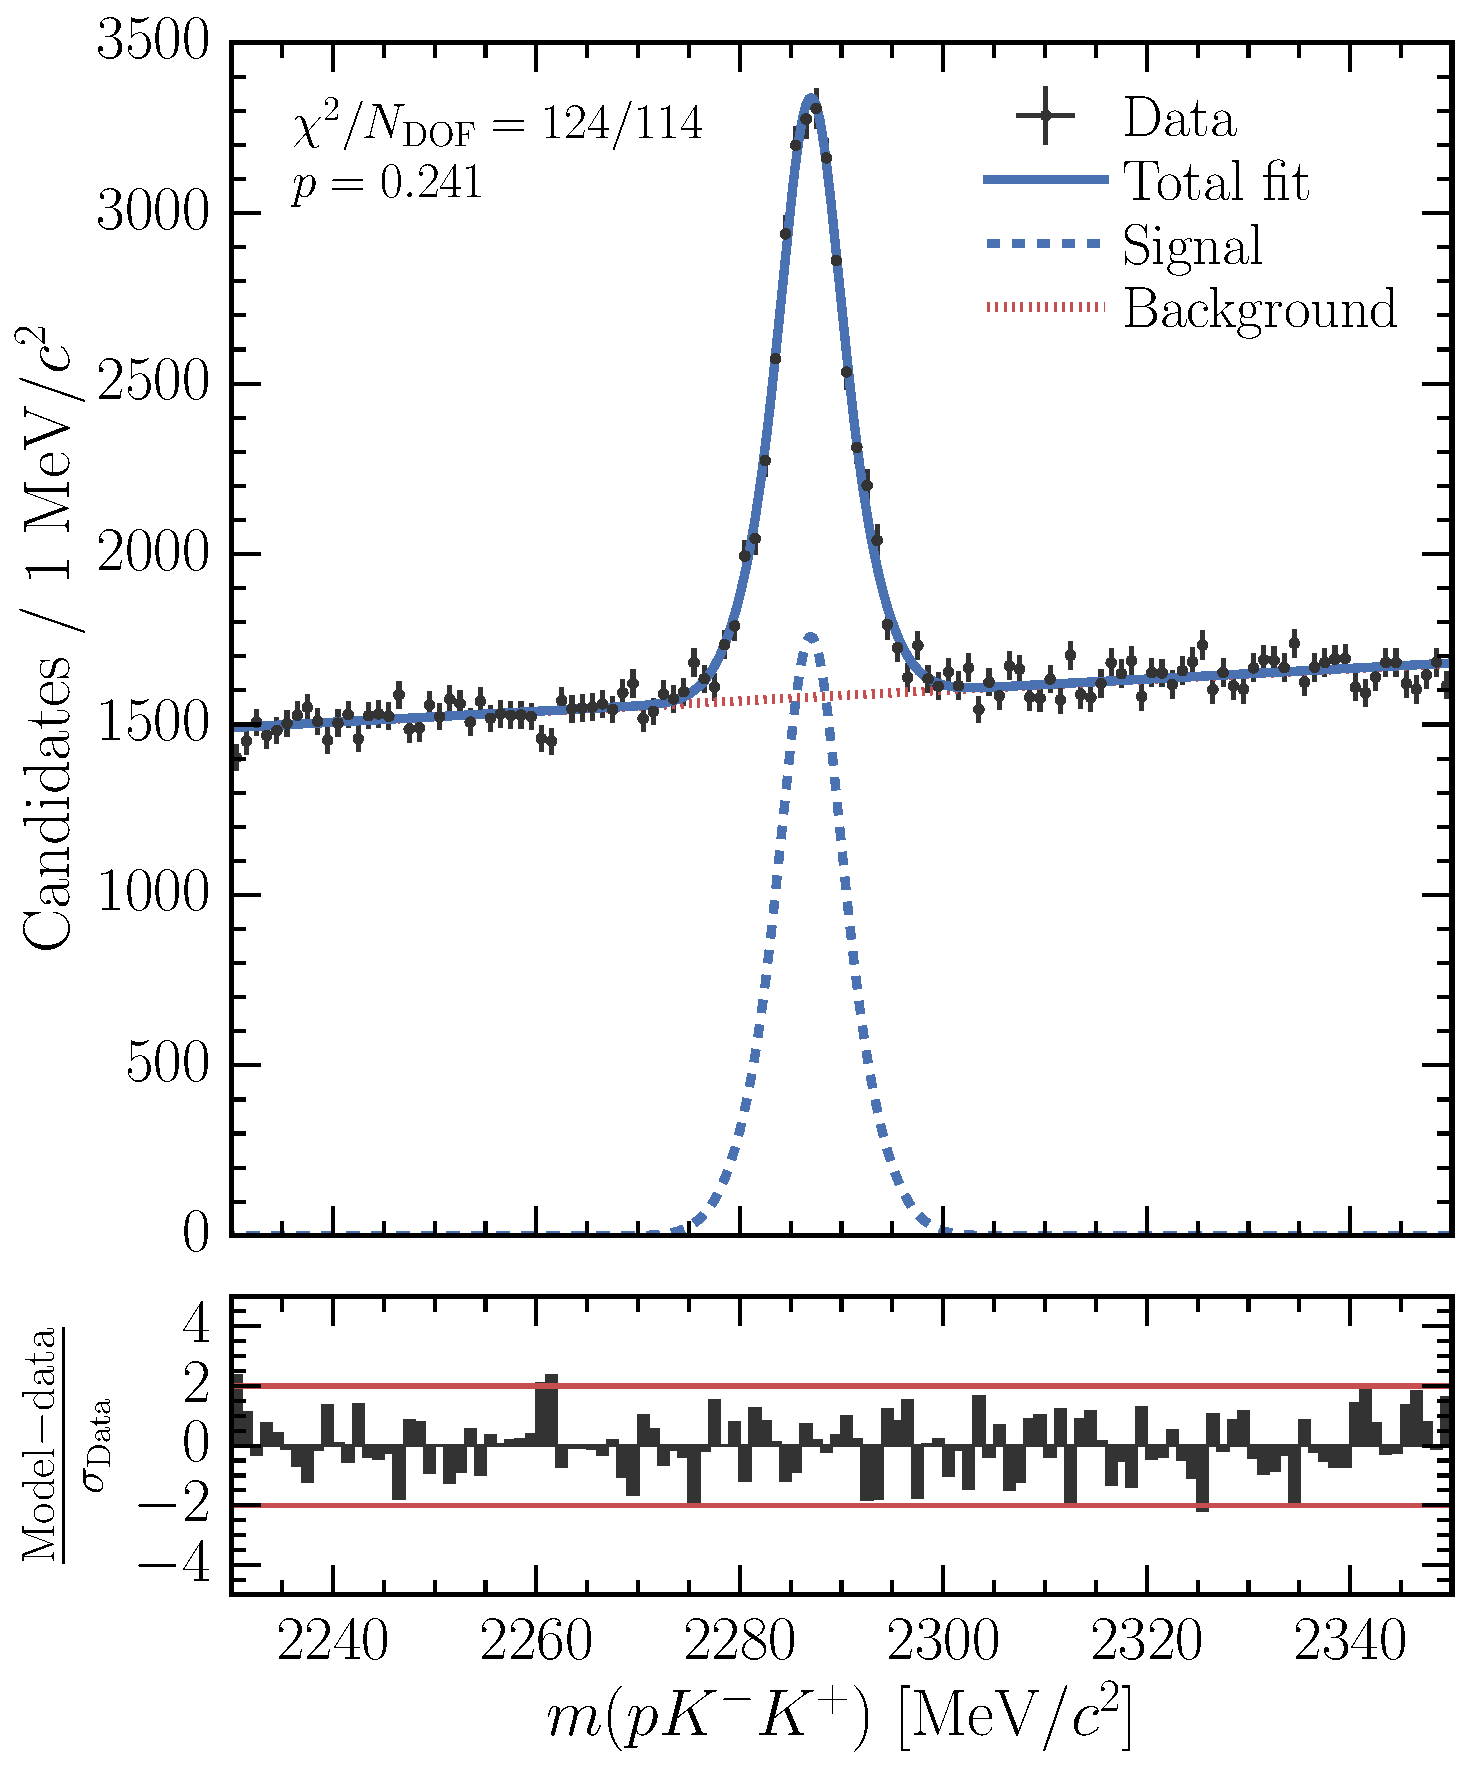
\includegraphics[width=\textwidth]{cpv/preliminary_fits/fits-unweighted_no-simultaneous/LcTopKK_2012_MagDown_fit.pdf}
    \caption{\pKK}
    \label{fig:cpv:prelim_fits:full:pKK}
  \end{subfigure}
  \begin{subfigure}[b]{0.5\textwidth}
    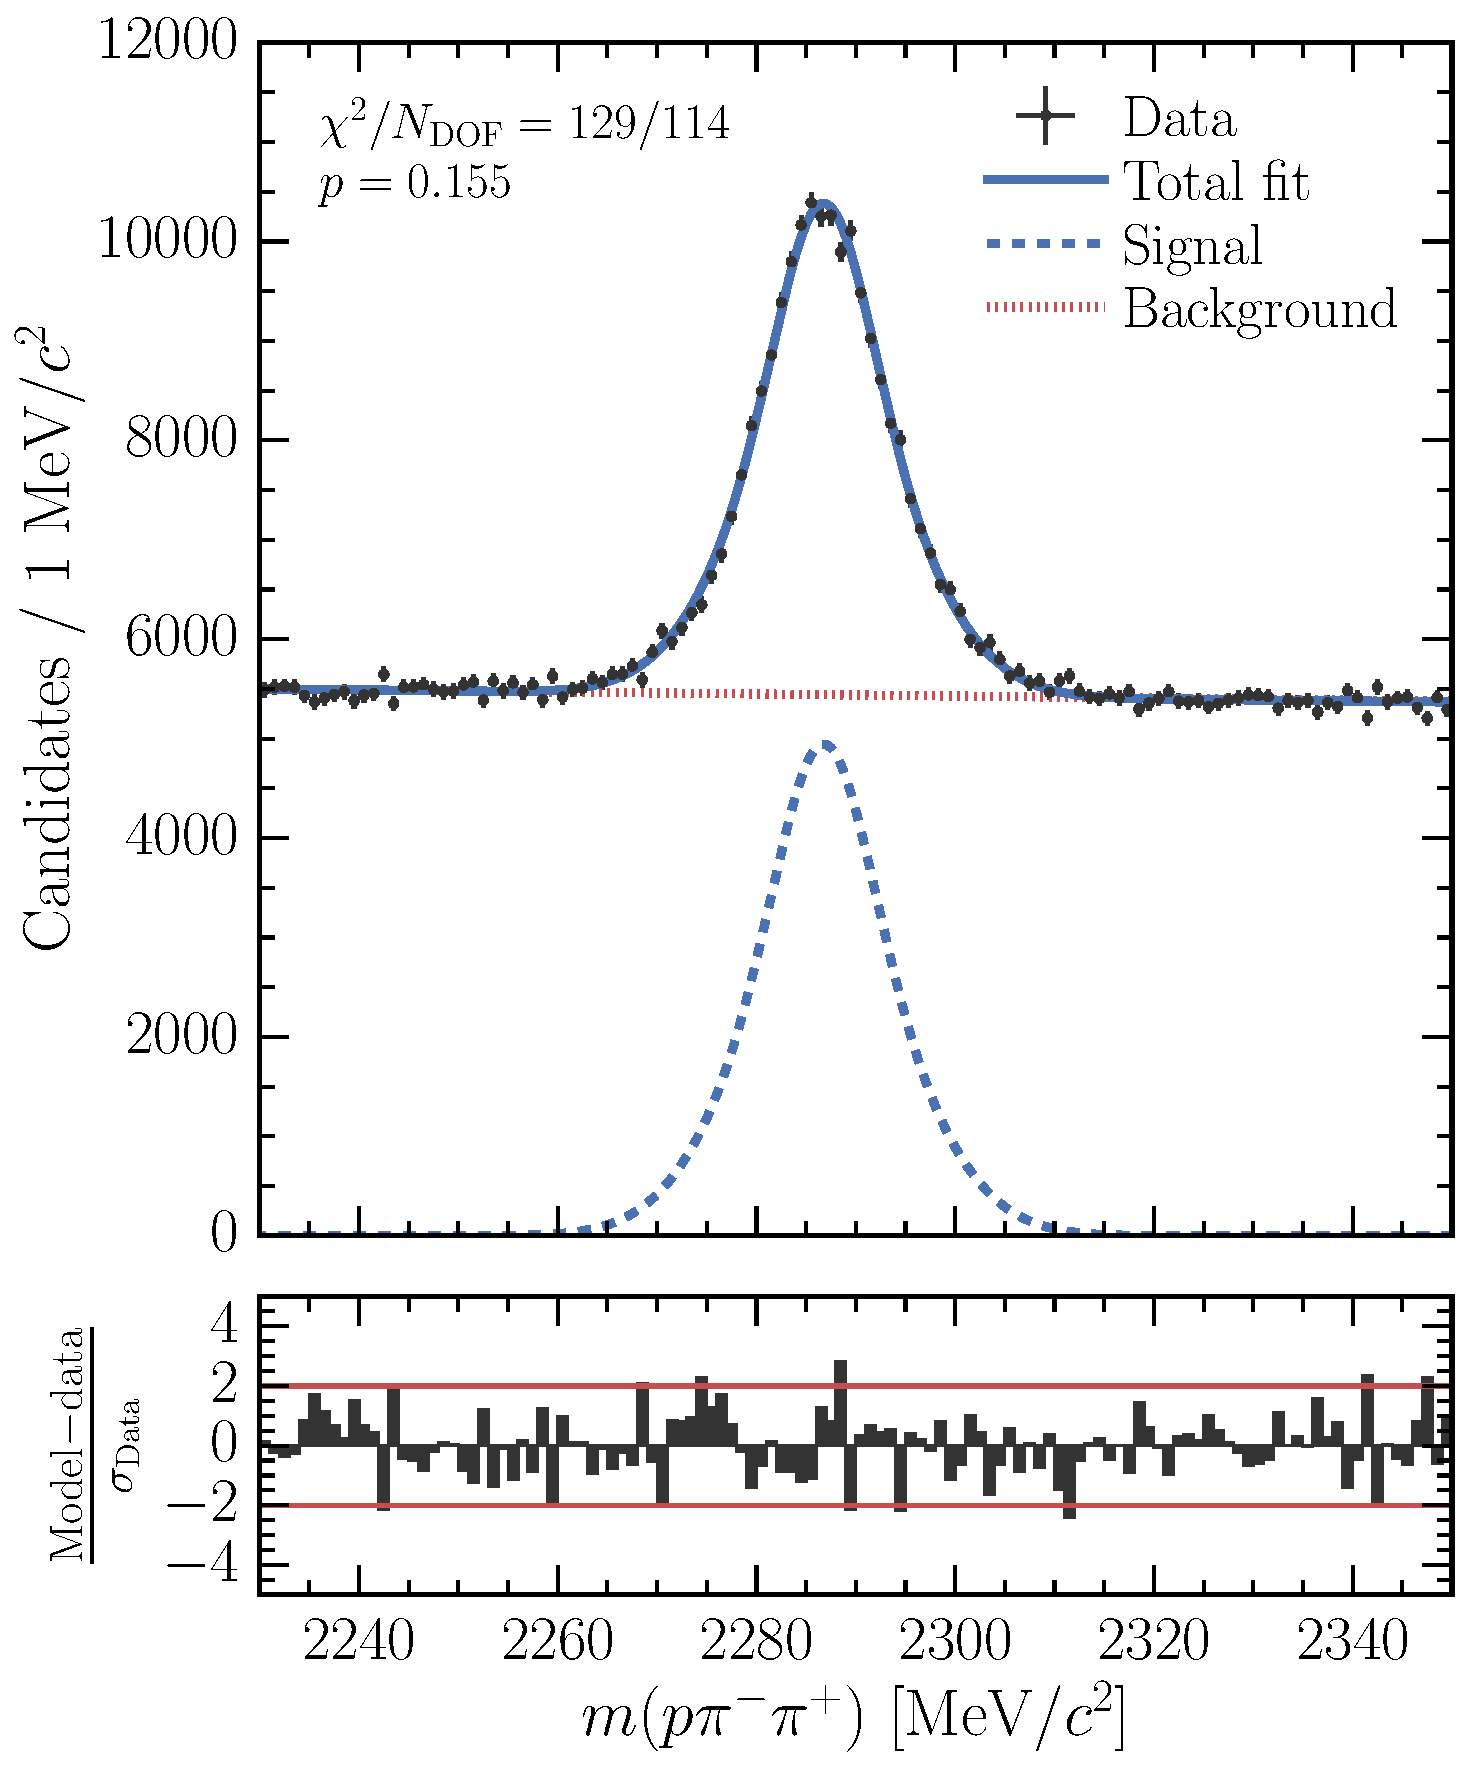
\includegraphics[width=\textwidth]{cpv/preliminary_fits/fits-unweighted_no-simultaneous/LcToppipi_2012_MagDown_fit.pdf}
    \caption{\ppipi}
    \label{fig:cpv:prelim_fits:full:ppipi}
  \end{subfigure}
  \caption{%
    Fits to the \PLambdac\ mass spectrum in the 2012 magnet down dataset for 
    \pKK~(\subref*{fig:cpv:prelim_fits:full:pKK}) and 
    \ppipi~(\subref*{fig:cpv:prelim_fits:full:ppipi}).
    The full offline selection is applied.
    The solid blue line is the total fit to the data in black points, and the 
    dotted red and dashed blue lines are the background and signal components, 
    respectively.
    Below each fit is a pull plot, showing the difference between the total fit 
    model and the data in each bin, normalised by the Poisson uncertainty on 
    the number of entries in that bin.
  }
  \label{fig:cpv:prelim_fits:full}
\end{figure}

\begin{figure}
  \begin{subfigure}[b]{0.5\textwidth}
    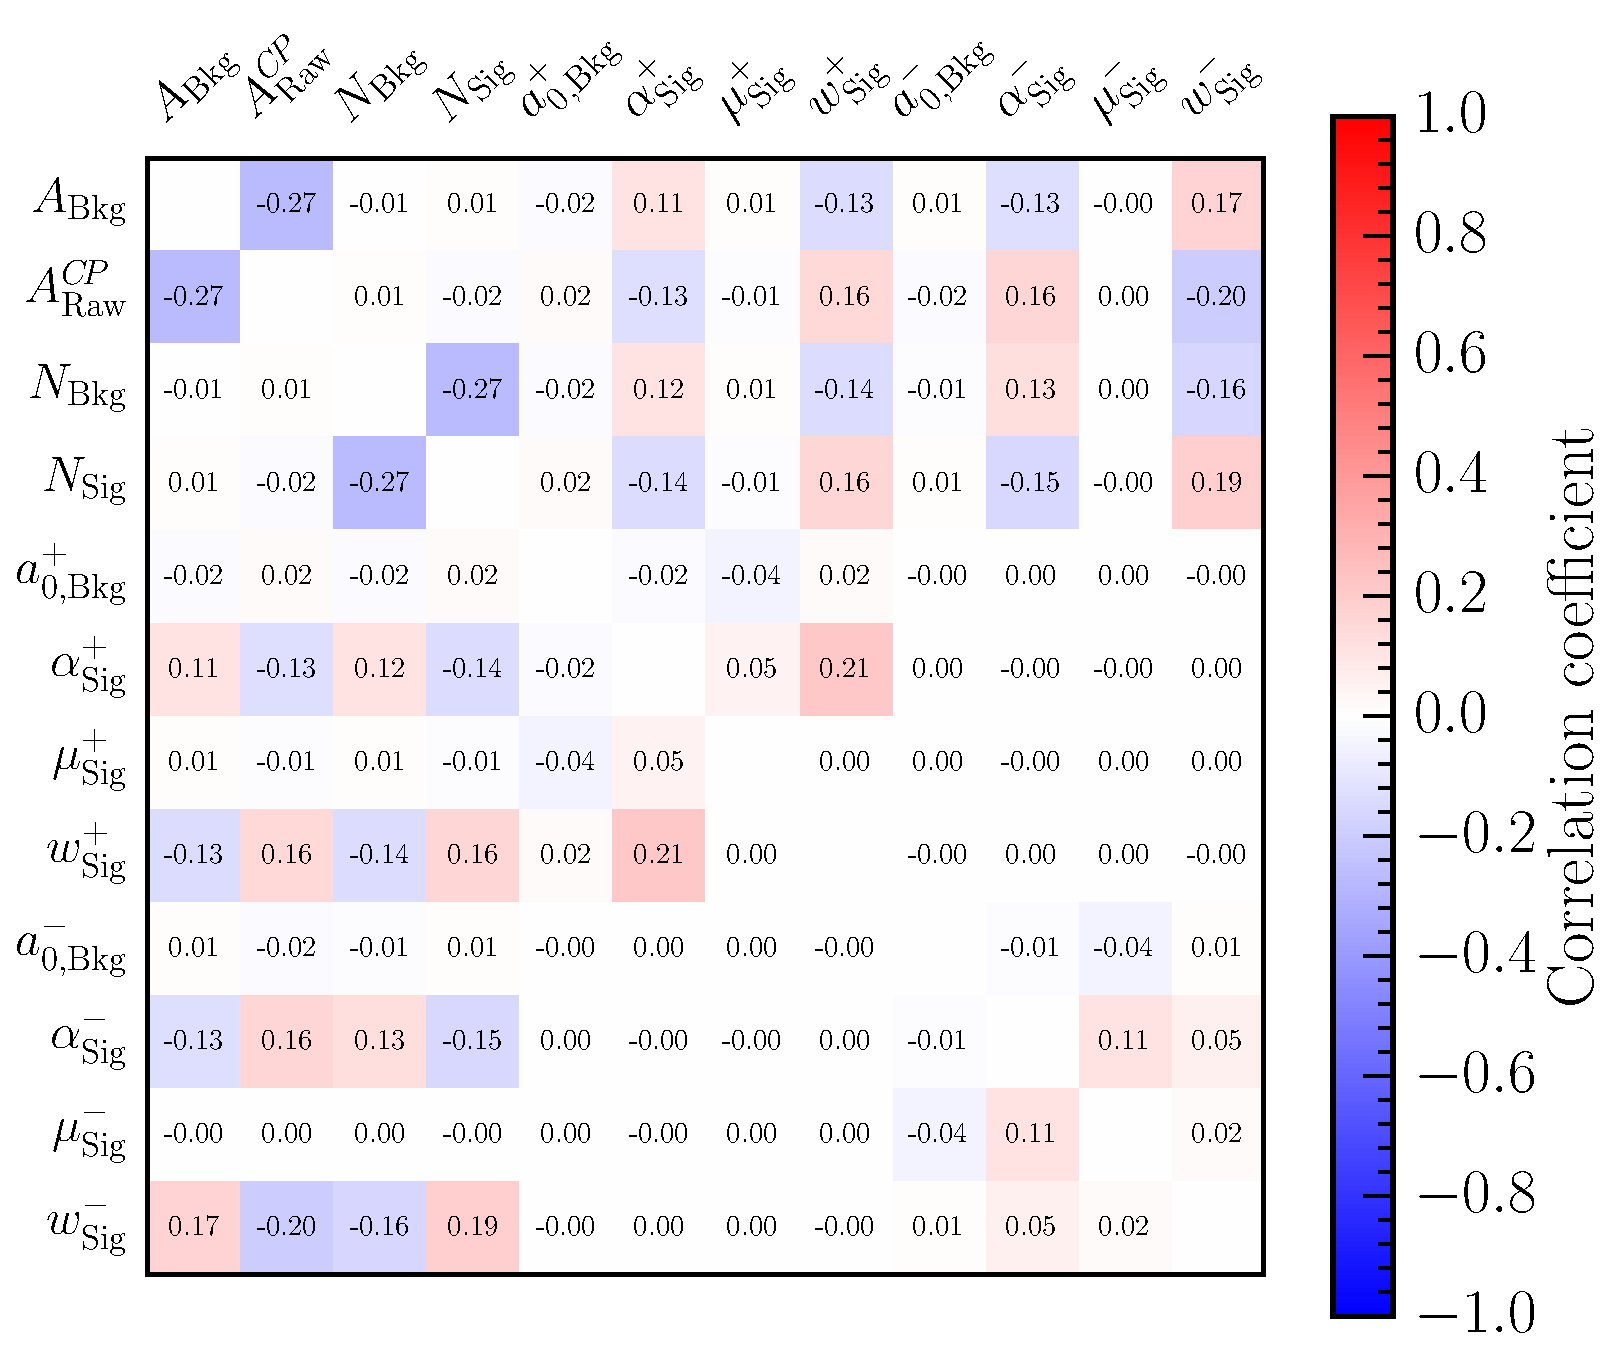
\includegraphics[width=\textwidth]{cpv/preliminary_fits/fits-unweighted_no-simultaneous/LcTopKK_2012_MagDown_correlation_matrix.pdf}
    \caption{\pKK}
    \label{fig:cpv:prelim_fits:full_correlation:pKK}
  \end{subfigure}
  \begin{subfigure}[b]{0.5\textwidth}
    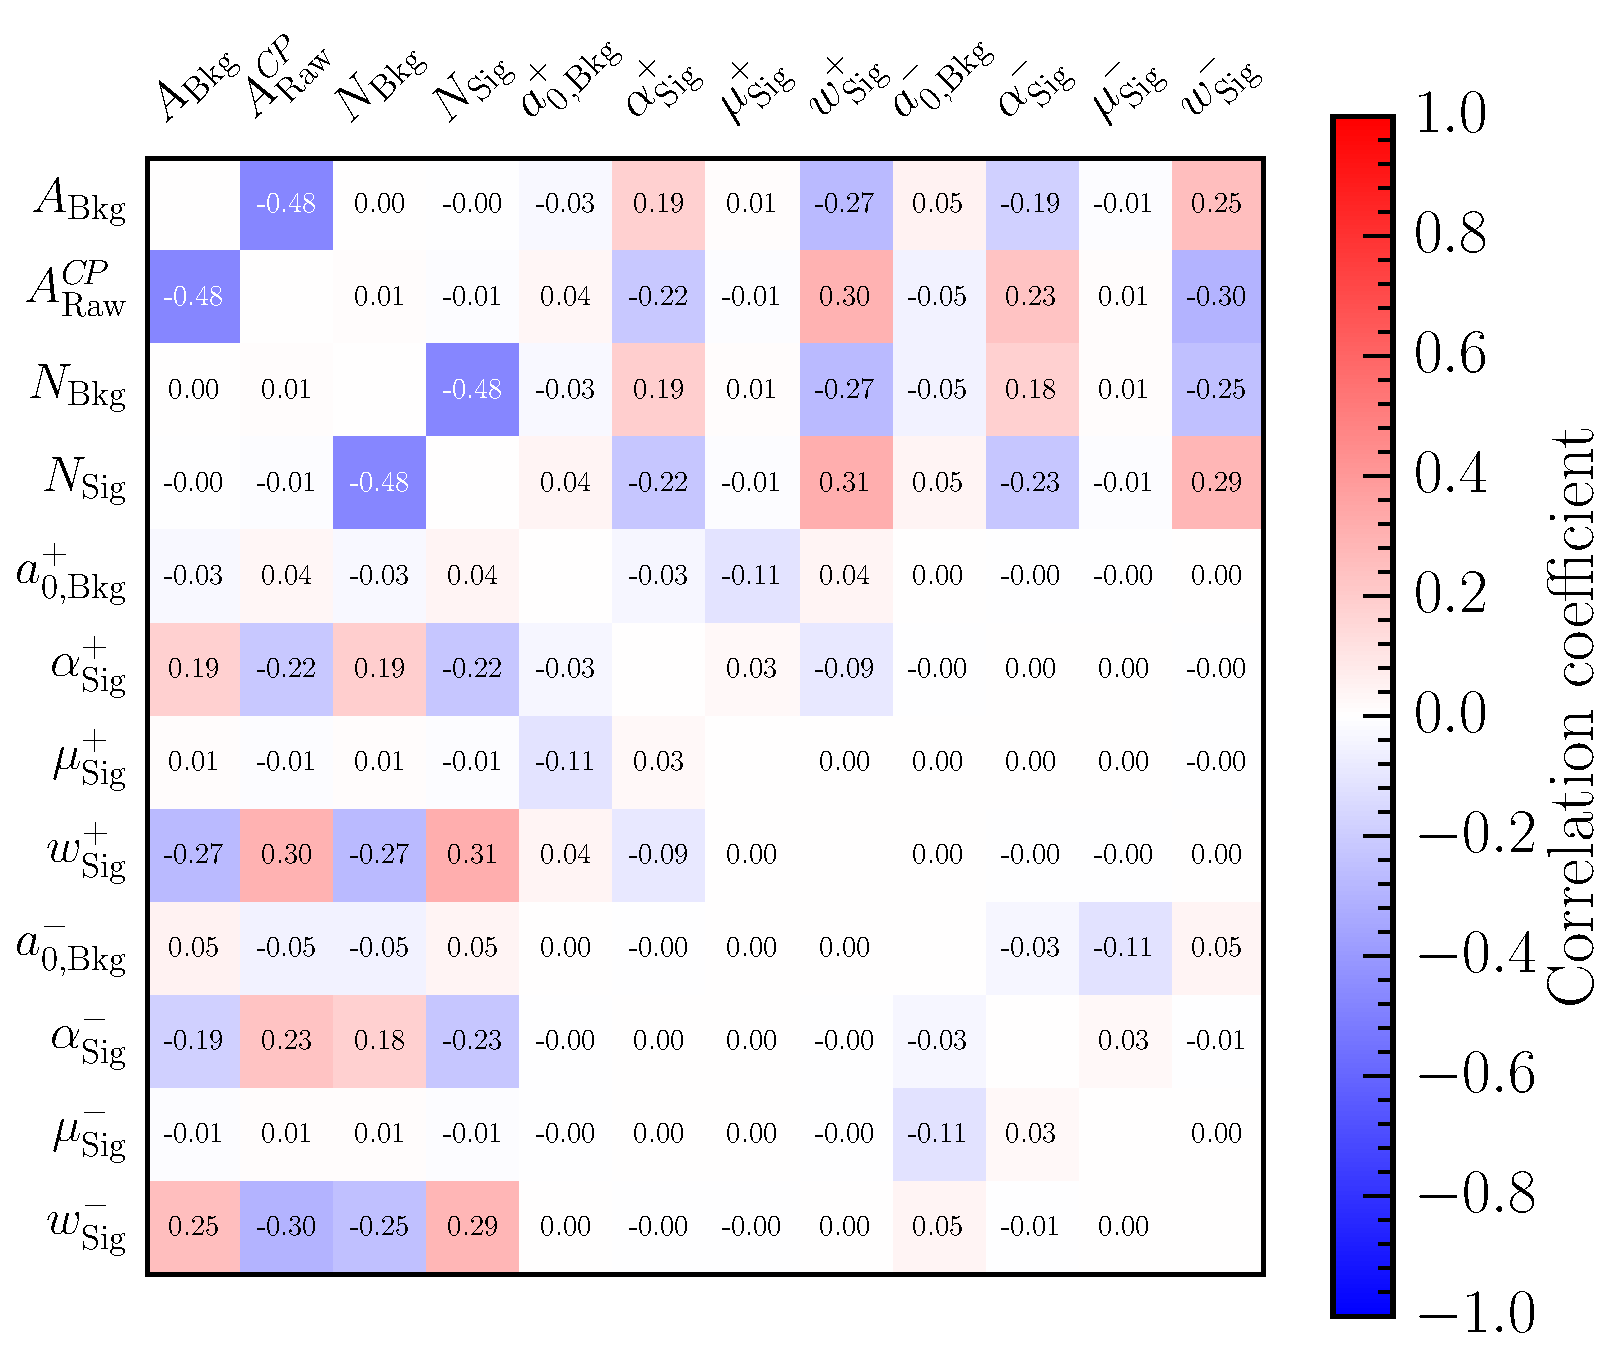
\includegraphics[width=\textwidth]{cpv/preliminary_fits/fits-unweighted_no-simultaneous/LcToppipi_2012_MagDown_correlation_matrix.pdf}
    \caption{\ppipi}
    \label{fig:cpv:prelim_fits:full_correlation:ppipi}
  \end{subfigure}
  \caption{%
    Correlation matrices for the fit parameters used in the fit to the 
    \PLambdac\ mass spectrum in the fully selected 2012 magnet down dataset for 
    \pKK~(\subref*{fig:cpv:prelim_fits:full_correlation:pKK}) and 
    \ppipi~(\subref*{fig:cpv:prelim_fits:full_correlation:ppipi}).
    The corresponding fits are shown in \cref{fig:cpv:prelim_fits:full}.
  }
  \label{fig:cpv:prelim_fits:full_correlation}
\end{figure}

\begin{table}
  \centering
  \caption{%
    Model parameters as determined in the preliminary fit to the 2012 magnet 
    down subset of the \pKK\ data.
  }
  \label{tab:cpv:prelim_fits:params:pKK}
  \begin{tabular}{cc}
  \toprule
  Parameter & Value \\
  \midrule
$a_{0,\mathrm{Bkg}}$ & $(-2.7 \pm 1.4) \times 10^{-2}$ \\
$\alpha_{\mathrm{Sig}}$ & $(74.3 \pm 1.7) \times 10^{-2}$ \\
$\mu_{\mathrm{Sig}}$ & $2286.992 \pm 0.05$ \\
$w_{\mathrm{Sig}}$ & $(321.6 \pm 4.3) \times 10^{-2}$ \\
$N_{\mathrm{Bkg}}$ & $(151.6 \pm 1.4) \times 10^{2}$ \\
$N_{\mathrm{Sig}}$ & $(92.5 \pm 1.2) \times 10^{2}$ \\
  \bottomrule
\end{tabular}
\end{table}

\begin{table}
  \centering
  \caption{%
    Model parameters as determined in the preliminary fit to the 2012 magnet 
    down subset of the \ppipi\ data.
  }
  \label{tab:cpv:prelim_fits:params:ppipi}
  \begin{tabular}{cc}
  \toprule
  Parameter & Value \\
  \midrule
$a_{0,\mathrm{Bkg}}$ & $(-90.8 \pm 5.9) \times 10^{-3}$ \\
$\alpha_{\mathrm{Sig}}$ & $(737.8 \pm 7.5) \times 10^{-3}$ \\
$\mu_{\mathrm{Sig}}$ & $2286.736 \pm 0.041$ \\
$w_{\mathrm{Sig}}$ & $(612.9 \pm 3.8) \times 10^{-2}$ \\
$N_{\mathrm{Bkg}}$ & $(884.5 \pm 3.9) \times 10^{2}$ \\
$N_{\mathrm{Sig}}$ & $(598.3 \pm 3.5) \times 10^{2}$ \\
  \bottomrule
\end{tabular}
\end{table}

\begin{table}
  \centering
  \caption{%
    Signal and background yields measured in the preliminary fit for each fully 
    selected subset of the \pKK\ data.
  }
  \label{tab:cpv:prelim_fits:yields:pKK}
  \begin{tabular}{ccccc}
  \toprule
  Year & Polarity & Signal yield (\nsig) & Background yield (\nbkg) & $\nsig/\mathcal{L}$ [\si{\pico\barn}] \\
  \midrule
2011   & Down     & $3,930 \pm 80$       & $6,670 \pm 90$           & $7.0 \pm 0.2$                         \\
2011   & Up       & $2,850 \pm 70$       & $4,710 \pm 80$           & $6.8 \pm 0.2$                         \\
2012   & Down     & $9,250 \pm 120$      & $15,160 \pm 140$         & $9.3 \pm 0.2$                         \\
2012   & Up       & $8,990 \pm 110$      & $15,370 \pm 140$         & $9.0 \pm 0.2$                         \\
  \bottomrule
\end{tabular}

\end{table}

\begin{table}
  \centering
  \caption{%
    Signal and background yields measured in the preliminary fit for each fully 
    selected subset of the \ppipi\ data.
  }
  \label{tab:cpv:prelim_fits:yields:ppipi}
  \begin{tabular}{ccccc}
  \toprule
  Year & Polarity & \nsig            & \nbkg            & $\nsig/\mathcal{L}$ [\si{\pico\barn}] \\
  \midrule
2011   & Down     & $25,040 \pm 220$ & $34,060 \pm 240$ & $44.4 \pm 0.9$                        \\
2011   & Up       & $18,370 \pm 190$ & $24,360 \pm 210$ & $43.5 \pm 0.9$                        \\
2012   & Down     & $59,830 \pm 350$ & $88,450 \pm 390$ & $60.3 \pm 0.8$                        \\
2012   & Up       & $57,460 \pm 340$ & $89,670 \pm 390$ & $57.4 \pm 0.7$                        \\
  \bottomrule
\end{tabular}

\end{table}

\begin{figure}
  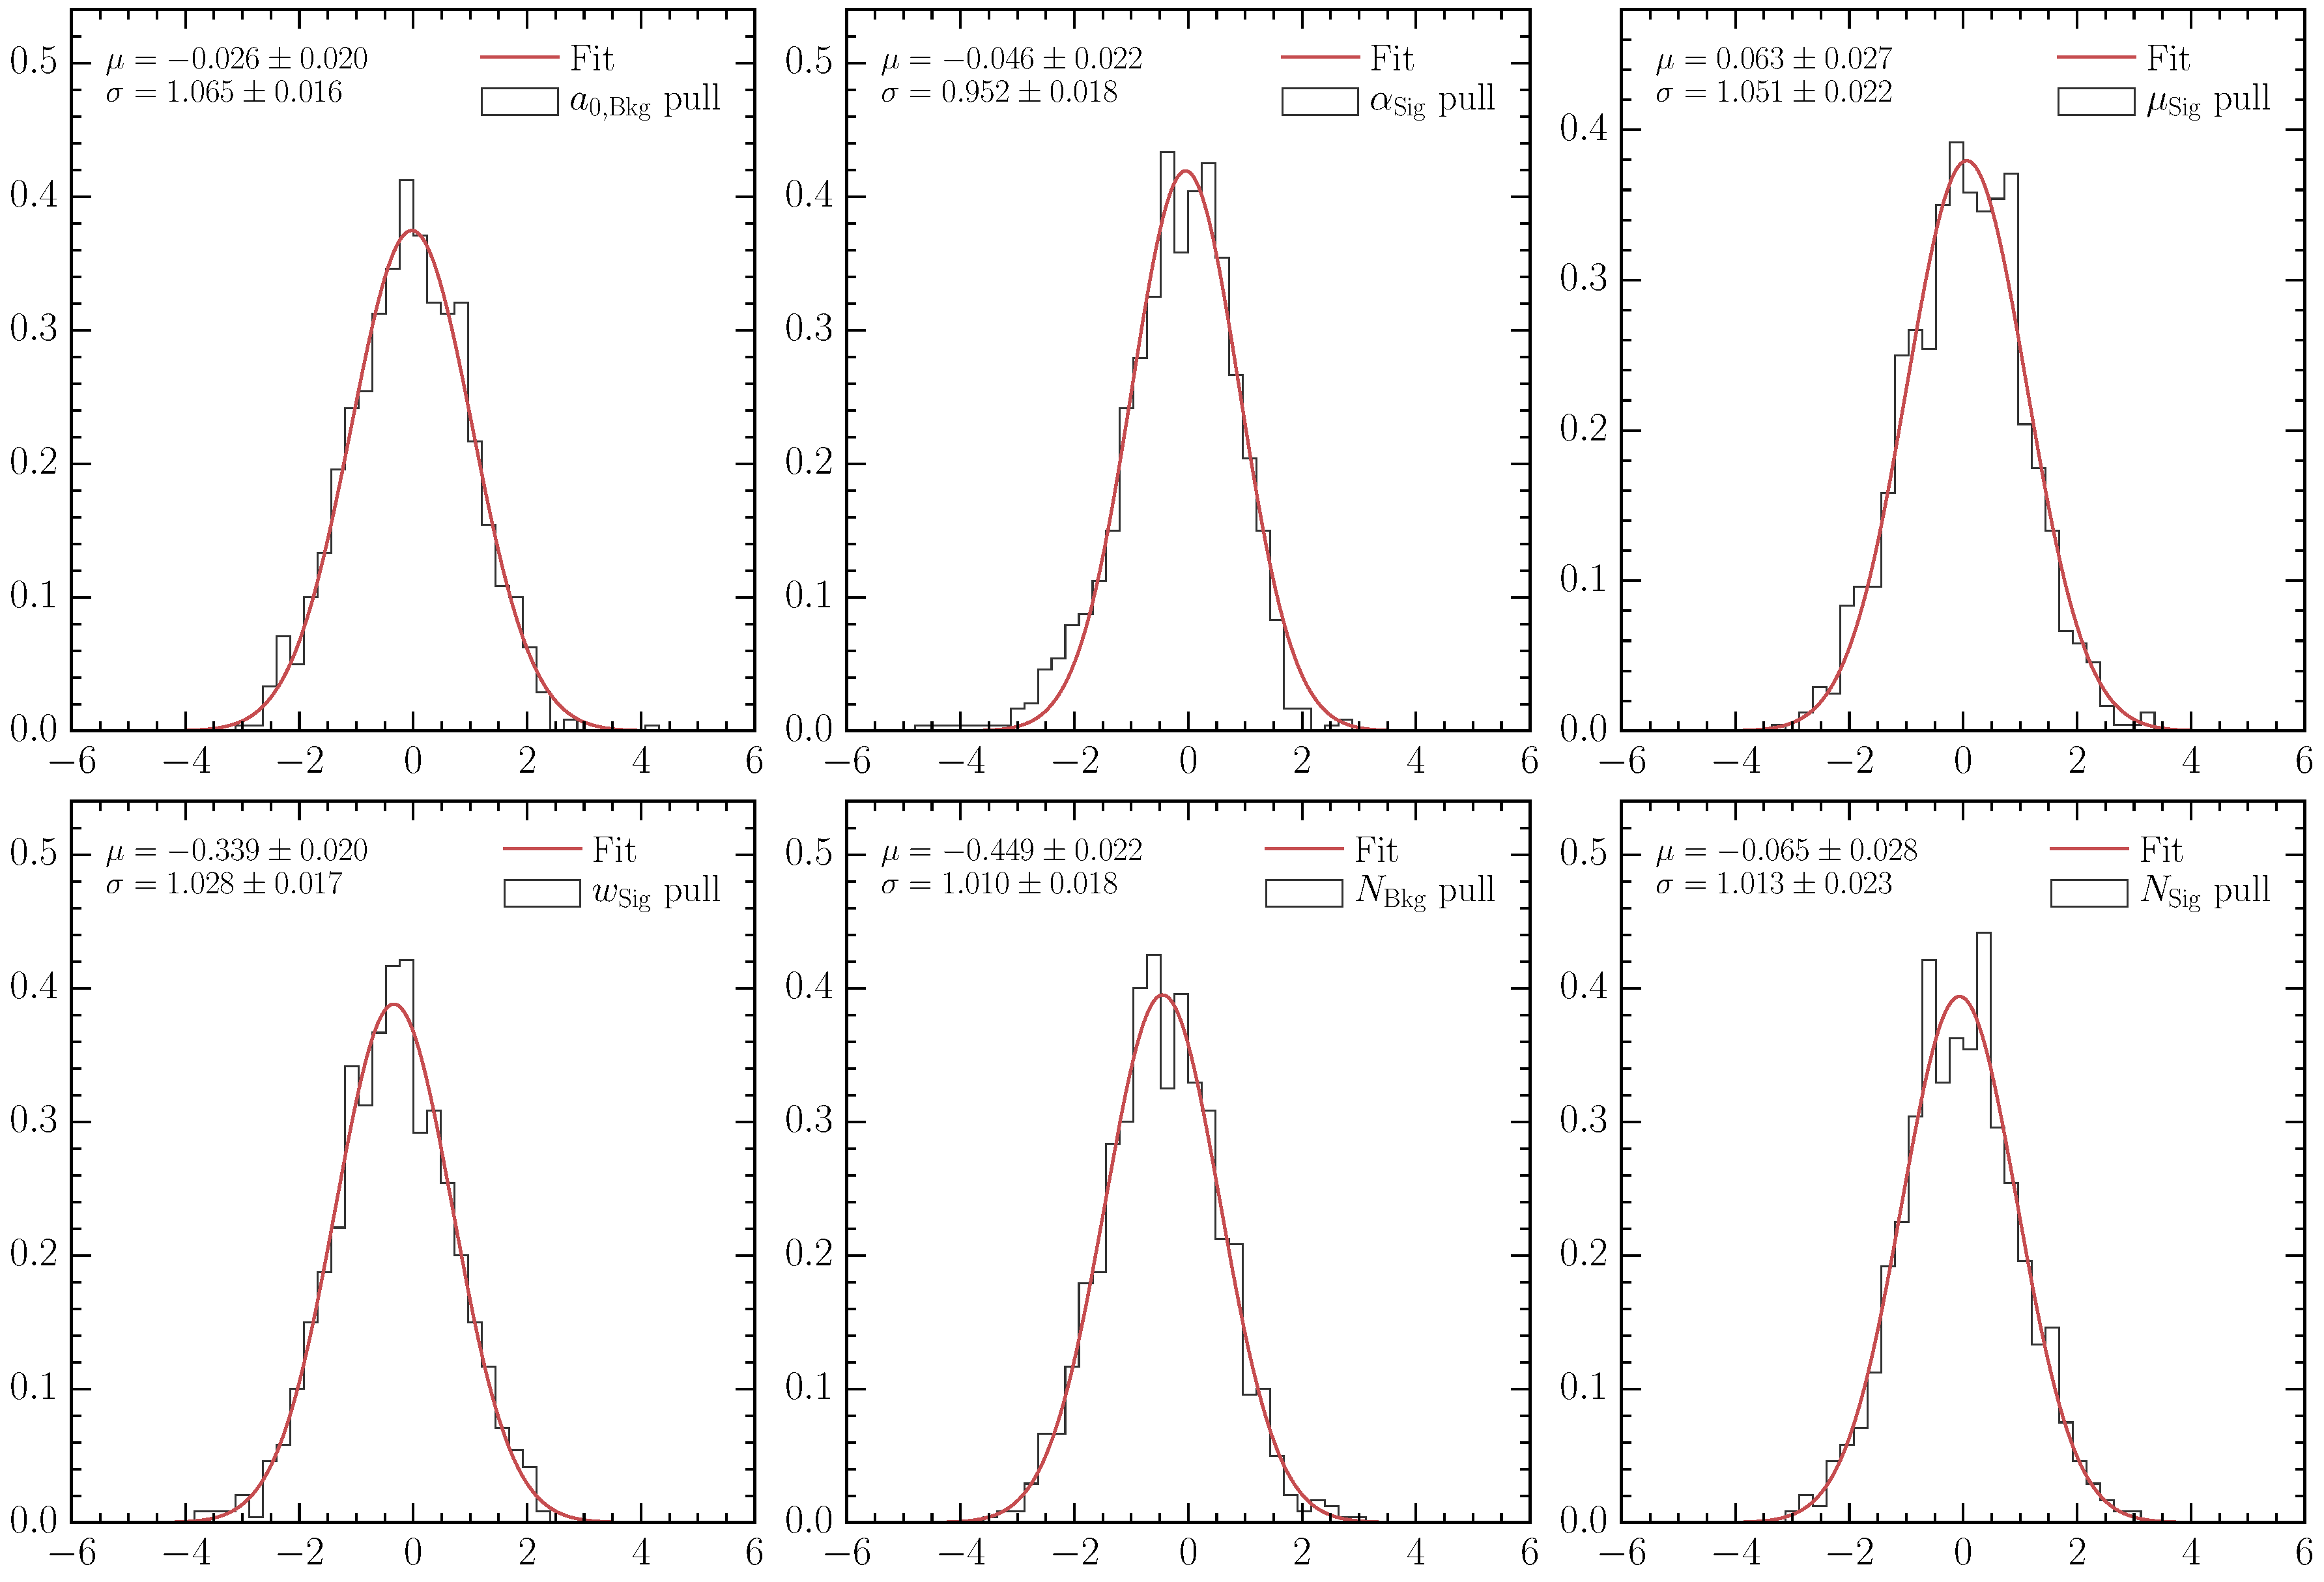
\includegraphics[width=\textwidth]{cpv/preliminary_fits/fits-unweighted_no-simultaneous/LcTopKK_2012_MagDown_pulls.pdf}
  \caption{%
    Validation of the fits to the \PLambdac\ mass spectrum in the 
    charge-combined 2012 magnet down \pKK\ dataset.
    Each plot shows the distribution of the pull values for a single fit 
    parameter, indicated in the legend, along with a fit of a Gaussian 
    distribution with mean $\mu$ and width $\sigma$.
  }
  \label{fig:cpv:prelim_fits:validation:pKK}
\end{figure}

\begin{figure}
  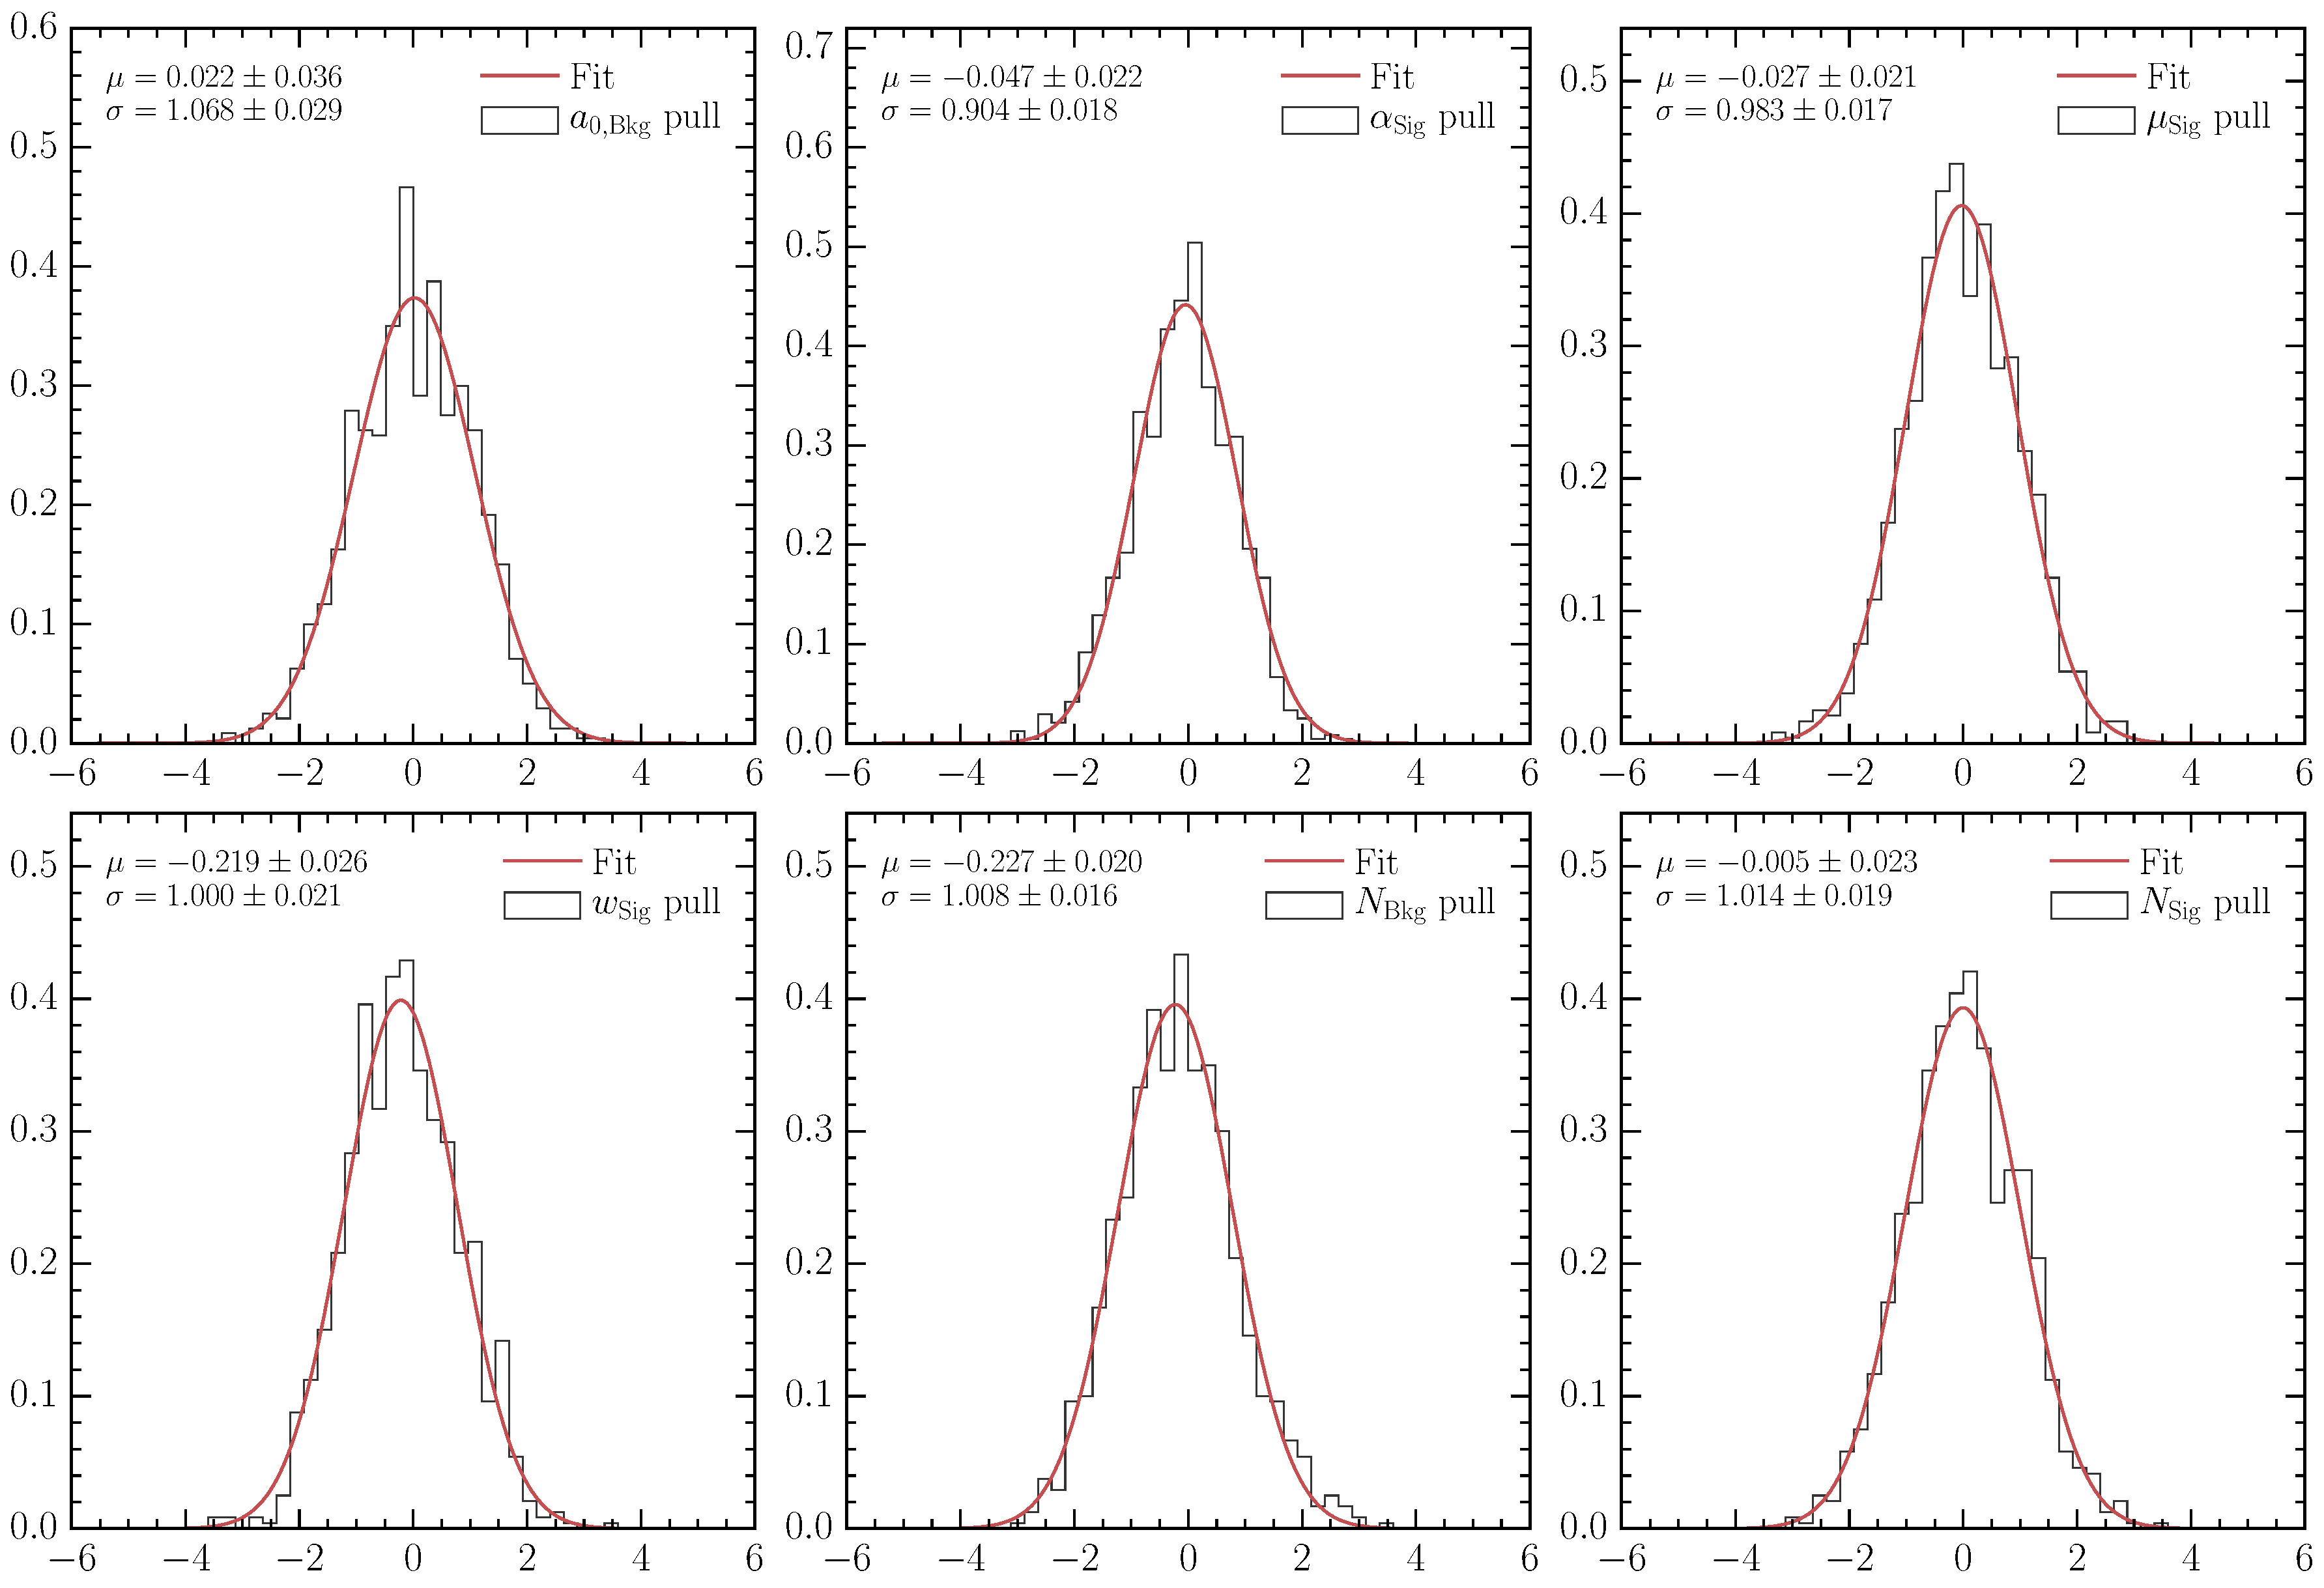
\includegraphics[width=\textwidth]{cpv/preliminary_fits/fits-unweighted_no-simultaneous/LcToppipi_2012_MagDown_pulls.pdf}
  \caption{%
    Validation of the fits to the \PLambdac\ mass spectrum in the 
    charge-combined 2012 magnet down \ppipi\ dataset.
    Each plot shows the distribution of the pull values for a single fit 
    parameter, indicated in the legend, along with a fit of a Gaussian 
    distribution with mean $\mu$ and width $\sigma$.
  }
  \label{fig:cpv:prelim_fits:validation:ppipi}
\end{figure}
